\chapter{Introducción}
\section{Definición del problema}\label{def_problem}
El problema de la selección de características se define como el proceso de
seleccionar un subconjunto de características relevantes~\cite{miao_survey_2016}. Una característica es
una propiedad individual medible de un fenómeno concreto. Este problema es
considerado un problema \textbf{NP duro}~\cite{leeuwen_algorithms_1998,johnjeffery_automata}. La reducción de dimensionalidad, y con
ello de características, suele ser necesario a la hora de crear un modelo predictivo por medio
del aprendizaje automático ya que muchas de las características
dentro de un conjunto de datos pueden no llegar a ser relevantes para solucionar
aquellos problemas que se intentan solucionar, ya sea por que no aporta información,
porque puede ser agrupada junto a otras tantas en una sola propiedad o incluso porque hay ruido
en los datos, lo cual es inevitable~\cite{Mostafa2012}.\\[6pt]
Gracias a la reducción de características es posible mejorar tanto la capacidad de generalización
como la precisión del modelo predictivo gracias a la reducción de \textit{ruido}.\\[6pt]
Siendo $f$ la función objetivo a predecir, $H^n$ el conjunto de hipótesis o conjunto de modelos
de dimensión $n$ posibles, $h^*(x)$ el mejor modelo aprendido y $x$ una variable de entrada. El ruido conocido
como ruido estocástico es aquel que atiende a una variación aleatoria que
puede surgir de diversos factores, como mediciones imprecisas de señales o la falta de
precisión en sensores. Por otro lado, el ruido determinista está directamente
relacionado con la complejidad de un modelo. Su presencia aumenta la probabilidad de
sobreajuste. El ruido determinista puede explicarse como la parte de la función $f$ que el conjunto
de hipótesis $H^n$ no puede capturar, es decir, $f(x) - h^*(x)$. Este tipo de ruido se
considera así porque la función (modelo) no es lo suficientemente compleja como para comprender
esa parte. Este ruido depende de $H^n$ y permanece constante para un valor dado de $x$~\cite{Mostafa2012}.\\[6pt]
La reducción de características ayuda a manejar ambos tipos de ruido~\cite{miao_survey_2016,Mostafa2012} al simplificar el
modelo, lo que puede reducir el impacto del ruido estocástico y disminuir la complejidad del
modelo, lo que a su vez puede ayudar a mitigar el ruido determinista al mejorar la capacidad
del modelo para capturar las características relevantes y descartar las irrelevantes.
Esto puede conducir a una mejor capacidad de generalización y a una reducción del sobreajuste.\\[6pt]
Además de la simplificación del modelo, que conduce a una reducción del ruido, la
selección de características es un preprocesamiento necesario por varias razones:
\begin{enumerate}
      \item Interpretabilidad: La presencia de características
            irrelevantes puede complicar innecesariamente la interpretación y el
            rendimiento de los modelos de aprendizaje automático~\cite{miao_survey_2016}. La selección de un
            subconjunto relevante de características puede simplificar el modelo
            resultante, haciéndolo más comprensible y fácilmente interpretable.

      \item Mejora de la eficiencia computacional: La reducción de la
            dimensionalidad puede conducir a un ahorro significativo en términos de
            tiempo y recursos computacionales necesarios para el entrenamiento y la
            evaluación de modelos. Al eliminar características irrelevantes, se reduce
            la complejidad del problema y se acelera el proceso de aprendizaje.

      \item Evita la maldición de la dimensionalidad~\cite{venkat2018curse, bellman1957dynamic}: Cuando la dimensionalidad
            se incrementa en un problema, el volumen del espacio también lo hace, y esto ocurre
            tan rápido que  hace que los datos disponibles se vuelvan dispersos. De forma que para
            obtener un resultado seguro/fiable, la cantidad de datos necesitados debe verse
            incrementada de manera exponencial con la dimensionalidad~\cite{udacity2015curse}. A menor dimensionalidad
            (características en el conjunto de datos) menos datos harán falta para obtener un buen
            modelo.
\end{enumerate}
En este trabajo, se lleva a cabo una investigación y análisis comparativo entre varios métodos
de la familia \textbf{wrapper} o métodos de envoltura. Existen multitud de estrategias~\cite{miao_survey_2016}
que intentan dar solución a este problema. Los métodos de búsqueda más famosos son los de filtrado
(\textbf{filter}), los cuáles seleccionan las características más discriminativas según la naturaleza de los datos~\cite{miao_survey_2016}.
Por lo general, estos métodos realizan la selección de características antes de las tareas de clasificación y
agrupamiento. Ejemplos de algoritmos de filtrado son \textit{relieF}~\cite{kira_practical_1992} o F-statistic~\cite{ding_minimum_2005}.\\[6pt]
Los métodos \textbf{wrapper}, en cambio, utilizan el algoritmo de aprendizaje usado postprocesamiento
para evaluar las características y seleccionar así las más útiles~\cite{miao_survey_2016}.\\[6pt]
Los algoritmos clasificatorios de aprendizaje utilizados en este trabajo son \textit{SVM}~\cite{cortes_support-vector_1995}
y \textit{kNN}~\cite{fix_discriminatory_1989,cover_nearest_1967}, siendo las máquinas de vectores de
soporte un método robusto y eficiente y los vecinos más cercanos un método simple, interpretable
y muy eficaz. Se analizará el resultado entre ambos clasificadores entre otros muchos análisis comparativos.

\subsection{Motivación}
El reciente interés del problema de la selección de características en el ámbito de las
metaheurísticas en los últimos años es más que evidente. Puede comprobarse como en los
últimos años hay una tendencia en la publicación de artículos presentando nuevos métodos
metaheurísticos, mejores con respecto a los clásicos o incluso comparativas y análisis entre
distintos algoritmos.\\[6pt]

Esta crecimiento viene acompañado, sin embargo, de comparaciones que distan de ser objetivas
por varios motivos. Entre varios artículos se comparan algoritmos del mismo tipo con
soluciones y resultados muy variables entre sí a pesar de mismas configuraciones a la hora
de experimentar, artículos sin código referenciado, de forma que sea más fácil interpretar
los resultados o duplicarlos, y algoritmos novedosos presentados por su autor o autores que
superanmal resto en alguna métrica concreta sin llegar a la rigurosidad adecuada.\\[6pt]

Por ello, la motivación principal de este trabajo es la de proveer información no sesgada y
todo lo objetiva posible por medio de un análisis comparativo entre los
algoritmos optimizatorios metaheurísticos más populares y más citados junto con los
algoritmos más robustos y clásicos en el campo de la optimización pseudo estocástica.

\subsection{Objetivos}
\textbf{Objetivo General:}

Realizar una comparación exhaustiva y objetiva de diversas metaheurísticas utilizadas en la
selección de características, con el propósito de proporcionar una visión integral y
evaluativa sobre su eficacia y aplicabilidad en diferentes contextos de análisis de
datos.\\[6pt]
\textbf{Objetivos Específicos:}

\begin{enumerate}
      \item Evaluar el desempeño de las metaheurísticas más relevantes en el ámbito de la
            selección de características, analizando métricas clave como precisión, estabilidad de
            las soluciones y eficiencia computacional. Se emplearán conjuntos de datos de referencia
            y metodologías de validación cruzada para garantizar la robustez de los resultados.

      \item Investigar la transferibilidad de las técnicas diseñadas para dominios continuos y
            binarios en el contexto de la selección de características. Se analizará si las
            metaheurísticas efectivas en un dominio son igualmente eficaces cuando se aplican a
            otro, identificando posibles ventajas y limitaciones de cada enfoque.

      \item Identificar las fortalezas y debilidades de cada metaheurística según el tipo de
            representación de las características. Se realizará un análisis detallado del
            comportamiento de las técnicas en problemas de selección de características con
            diferentes tipos de datos, destacando su rendimiento relativo y sus áreas de aplicación
            más adecuadas.

      \item Proporcionar recomendaciones prácticas basadas en los resultados obtenidos, con el
            objetivo de orientar a practicantes y académicos en la selección y aplicación de
            metaheurísticas en problemas reales de selección de características.

      \item Evaluar los resultados de las metaheurísticas en problemas de selección de característica
            usando distintos como algoritmos de aprendizaje los métodos \textit{kNN} y \textit{SVM}. Se realizará
            una comparativa a nivel de eficiencia en tiempo, estabilidad y calidad de los resultados.
\end{enumerate}

\subsection{Planificación}
Un trabajo de fin de grado consta de $12$ créditos ECTS, donde se estima que cada crédito debe valer unas $25$ horas de trabajo aproximadamente. Teniendo en cuenta estos datos, se calcula que la duración del TFG no debería ser superior a $300$ horas. Ha de tenerse en cuenta también que el alumno trabaja $25$ horas semanales y debe superar algunas asignaturas además de su projecto final para terminar la carrera. Por lo tanto, el proyecto se planifica con una duración extendida en el tiempo, pero con una carga de trabajo semanal menos intensiva.\\[6pt]
Se planifica una duración de $5$ meses aproximadamente. Se utilizará un diagrama de Gantt~\cite{Clark1922} para describir la planificación del proyecto, de manera que se realizarán tareas en un orden cronológico. Sin embargo, se reconoce que algunas tareas probablemente requerirán iteraciones posteriores, ya que es probable que se mejore y perfeccione el proyecto a lo largo de su ciclo de vida.\\[6pt]
Las fases del ciclo de vida son:
\begin{itemize}
      \item \textbf{Investigación inicial}
            Esto incluye investigar sobre conceptos básicos ya aprendidos, en forma de repaso sobre conceptos generales de aprendizaje automático, tipos de metaheurísticas, tipos de codificación, optimización de funciones, test estadísticos y conceptos básicos, código Python y librerías asociadas, instalación de estas a partir de un entorno virtual, configuración del entorno de trabajo e investigación sobre el problema de selección de características.

      \item \textbf{Diseño del software}: Planificación de la estructura general del código, uso de patrones de diseño que puedan ser de utilidad de cara a al mantenimiento del software a lo largo del desarrollo, concepto de modularización inicial del código (estructura del proyecto), uso de entornos virtuales.
      \item \textbf{Investigación metaheurísticas}: Realización de un estudio más exhaustivo acerca de las metaheurísticas a implementar y sus diferentes versiones binarias. Esto incluye un listado de 12 metaheurísticas, siendo estas:
            \begin{itemize}
                  \item Binary Firefly Algorithm
                  \item Binary Whale Optimization Algorithm
                  \item Binary Bat Swarm Optimizer
                  \item Binary Grey Wolf Optimizer
                  \item Binary Dragonfly Algorithm
                  \item Binary Grasshoper Algorithm
                  \item Binary Cuckoo Search
                  \item Binary Differential Algorithm
                  \item Ant Colony Optimization
                  \item Binary Artificial Bee Colony Optimization
                  \item Binary Particle Swarn Optimization
                  \item Genetic Algorithm (binary \& real)
            \end{itemize}
            De cada una de ellas se investigará su inspiración, funcionamiento, implementación y versiones binarias, normalmente asociadas al problema de selección de características.
      \item \textbf{Implementación del software}: Una vez claros los requisitos programáticos quedan establecidos, se implementará el software base. Esto incluye código en Python para la generación de gráficas, manejo de datasets en formato \textit{arff}, codificación de los algoritmos metaheurísticos en versión binaria, implementación de función objetivo (\textit{fitness}) y parametrización del programa para distintas pruebas.
      \item \textbf{Pruebas y refactorizado}: En esta etapa se llevarán a cabo pruebas exhaustivas para verificar la robustez y eficacia de los diferentes algoritmos implementados. Además, se considerará la refactorización del código si es necesario, con el fin de mejorar su estructura, claridad y mantenibilidad.
      \item \textbf{Análisis de resultados}: En esta fase se recopilarán datos de la ejecución de los algoritmos en sus diferentes versiones, así como entre ellos, utilizando los conjuntos de datos seleccionados para el proyecto. Esta recopilación de métricas permitirá una evaluación del rendimiento y la eficacia de cada algoritmo en comparación con los demás, así como su comportamiento en diferentes conjuntos de datos.
      \item \textbf{Documentación}: En esta etapa final se generará una documentación del proyecto que incluirá de forma general la descripción del problema, los objetivos, planificación, implementación, resultados y pruebas.
\end{itemize}

\begin{figure}[H]
      \begin{center}
            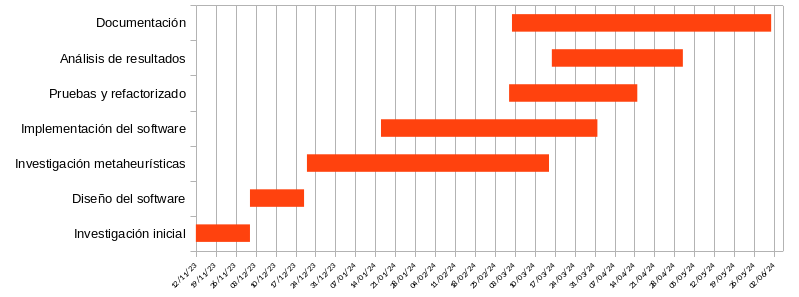
\includegraphics[width=1\textwidth]{imagenes/gantt-init.png}
      \end{center}
      \caption{Diagrama de Gantt inicial}
\end{figure}

La planificación inicial tiene en cuenta un curso ideal del ciclo de vida del proyecto, siendo las estapas más extensas la de creación del software e implementación de la documentación. Son etapas excluyentes, no pueden ocurrir a la vez según este tipo de planificación. Al terminar una etapa se pasa inmediatamente a la siguiente.\\[6pt]
La planificación final del proyecto se ha modificado significativamente debido a una serie de contratiempos y obstáculos surgidos durante su desarrollo, así como la influencia de numerosos eventos externos que han afectado a su cronograma. En particular, se han experimentado retrasos y bloqueos que han incidido en la duración prevista del proyecto. Por ejemplo, las etapas de implementación del software y la investigación de las metaheurísticas se han entrelazado debido a que la implementación efectiva del algoritmo se facilitaba una vez que se había estudiado a fondo la metaheurística correspondiente. Esto ha llevado a una reevaluación de la estrategia de planificación original, reconociendo que no habría sido eficiente estudiar todas las metaheurísticas simultáneamente y luego proceder con su implementación.

\begin{figure}[H]
      \begin{center}
            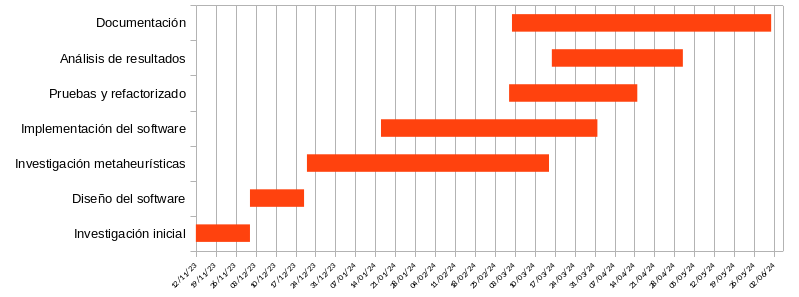
\includegraphics[width=1\textwidth]{imagenes/gantt-init.png}
      \end{center}
      \caption{Diagrama de Gantt final}
\end{figure}

El coste estimado del proyecto se divide en varios subcostes:
\begin{itemize}
      \item \textbf{Sueldo}: Considerando un precio de proyecto que deba cubrir gastos y compensar, se estima un salario por investigador de $52.000$€ al año, es decir, $25$€/hora. Al durar el proyecto aproximadamente $8$ meses, el salario final total es de $34.000$€.
      \item \textbf{Ordenador portátil}: El estudiante consta con un portátil HP HP Pavilion Laptop 14-ec0xxx como herramienta principal de trabajo, con un precio de $1000$€. Ha sido usado durante unos $8$ meses aproximadamente. Si se tiene en cuenta que la vida media de un portátil es de aproximadamente $4-5$ años~\cite{woidasky_use_2021} entonces el costo del ordenador sería de $133.3$€.
      \item \textbf{Servidor} Para la experimentación del proyecto se ha hecho uso de un servidor para ejecutar las distintas pruebas de los algoritmos. Se estima el precio por mes y total dada una estimación de los servicios de \textit{Google Cloud - Compute Engine}.
\end{itemize}
\begin{table}[H]
      \centering
      \begin{tabular}{|c|c|c|c|}
            \hline
            \textbf{Name}                            & \textbf{Quantity} & \textbf{Region} & \textbf{Service ID} \\
            \hline
            Compute optimized Core running in London & 150.0             & europe-west2    & 6F81-5844-456A      \\
            Compute optimized Ram running in London  & 600.0             & europe-west2    & 6F81-5844-456A      \\
            Storage PD Capacity in London            & 0.2               & europe-west2    & 6F81-5844-456A      \\
            \hline
      \end{tabular}
      \caption{Costos servidor Google Cloud - Part 1}
      \label{tab:server_costs_part1}
\end{table}
\begin{table}[H]
      \centering
      \begin{tabular}{|c|c|}
            \hline
            \textbf{SKU}   & \textbf{Total Price (USD)} \\
            \hline
            271A-7F2A-C5C5 & 6.56775                    \\
            0BD6-E233-D705 & 3.5202                     \\
            BF1A-6647-009D & 0.0096                     \\
            \hline
            Total Price:   & 10.09755                   \\
            \hline
      \end{tabular}
      \caption{Costos servidor Google Cloud - Part 2}
      \label{tab:server_costs_part2}
\end{table}
En la primera tabla, se detallan tres servicios distintos implementados en la región de Londres. Cada servicio se identifica por su nombre, cantidad (indicando la cantidad de recursos utilizados), región de implementación y un identificador único del servicio. Lo importante es que se ha calculado un servicio con $30$ vCPUs para paralelizar los trabajos.\\[6pt]

La segunda tabla complementa la primera proporcionando detalles adicionales sobre los servicios en términos de SKU (Stock Keeping Unit, una identificación única para un producto) y el precio total en dólares estadounidenses asociado con cada uno de ellos. El total, hecho el cambio de divisa a euros, es de $9.48$€ al mes, es decir, $75.84$€ en total (calculado para 8 meses).
Dado este desglose, se calcula el coste final del proyecto:
\begin{table}[h]
      \centering
      \begin{tabular}{|l|r|}
            \hline
            \textbf{Item}                    & \textbf{Costo (€)} \\ \hline
            Salario                          & 34.000             \\
            Ordenador portátil               & 133.3              \\
            Servidor CPU - GC Compute Engine & 75.84              \\
            \textbf{Total}                   & \textbf{34.209,14} \\ \hline
      \end{tabular}
      \caption{Costo estimado del proyecto}
      \label{tab:proyect_budget}
\end{table}